% Metódy inžinierskej práce

\documentclass[10pt,twoside,slovak,a4paper]{article}

\usepackage[slovak]{babel}
%\usepackage[T1]{fontenc}
\usepackage[IL2]{fontenc} % lepšia sadzba písmena Ľ než v T1
\usepackage[utf8]{inputenc}
\usepackage{graphicx}
\usepackage{url} % príkaz \url na formátovanie URL
\usepackage{hyperref} % odkazy v texte budú aktívne (pri niektorých triedach dokumentov spôsobuje posun textu)
\usepackage{float}
\usepackage{cite}
\usepackage{subcaption}
\usepackage{multicol}
\usepackage{atbegshi}
%\usepackage{times}

\pagestyle{headings}

\title{\thanks{}} % meno a priezvisko vyučujúceho na cvičeniach

\author{Jakub Žúbor\\[2pt]
	{\small Slovenská technická univerzita v Bratislave}\\
	{\small Fakulta informatiky a informačných technológií}\\
	{\small \texttt{xzubor@stuba.sk}}
	}

\date{\small október 2024} % upravte


\begin{document}
\AtBeginShipoutNext{\AtBeginShipoutUpperLeft{
  \hspace{3cm}\raisebox{-3cm}{
\includegraphics[width=4cm]{STU-FIIT-ncv.pdf}}}}

\maketitle

\begin{abstract}

Sociálne siete sa  v posledných rokoch stali populárnejšie ako kedykoľvek predtým. Za nárastom ich popularity stoja aj čoraz sofistikovanejšie algoritmy na zber a spracovanie informácií od užívateľov. Tieto algoritmy vytvárajú pre každého užívateľa jedinečný personalizovaný obsah na základe ich predošlých interakcií. Toto odporúčanie obsahu, ktorý je ušitý každému na mieru, môže viesť k vytvoreniu informačných bublín a podporovaniu rôznych stereotypov a ideológií ku ktorým konzumenti už predtým prejavovali sympatie, čo prispieva k polarizácii spoločnosti. \\
\\
V mojej práci sa budem venovať tomu, aké využite majú odporúčacie systémy na sociálnych sieťach, zberu dát a na čo sú tieto dáta využívané veľkými spoločnosťami, ako je napríklad Google, Facebook, Instagram, TikTok alebo X (v minulosti Twitter). Ďalej sa chcem takisto venovať dopadu odporúčacích systémov na spoločnosť a psychickú stránku jednotlivca (potenciál vzniku závislosti na sociálnych sieťach, FOMO – fear of missing out), a stratégiám, ktoré veľké spoločnosti používajú aby si získali a udržali našu pozornosť.\\
\\
Bez odporúčacích systémov a algoritmov by sociálne siete nemohli fungovať a tým že aj naďalej narastá ich popularita sa odporúčacie systémy za pomoci AI a strojového učenia viac a viac zdokonaľujú a dopad odporúčacích systémov bude naďalej rásť.

\end{abstract}



\section{Úvod}

\begin{figure}[H]
    \centering
    \begin{subfigure}{0.45\textwidth}
        \centering
        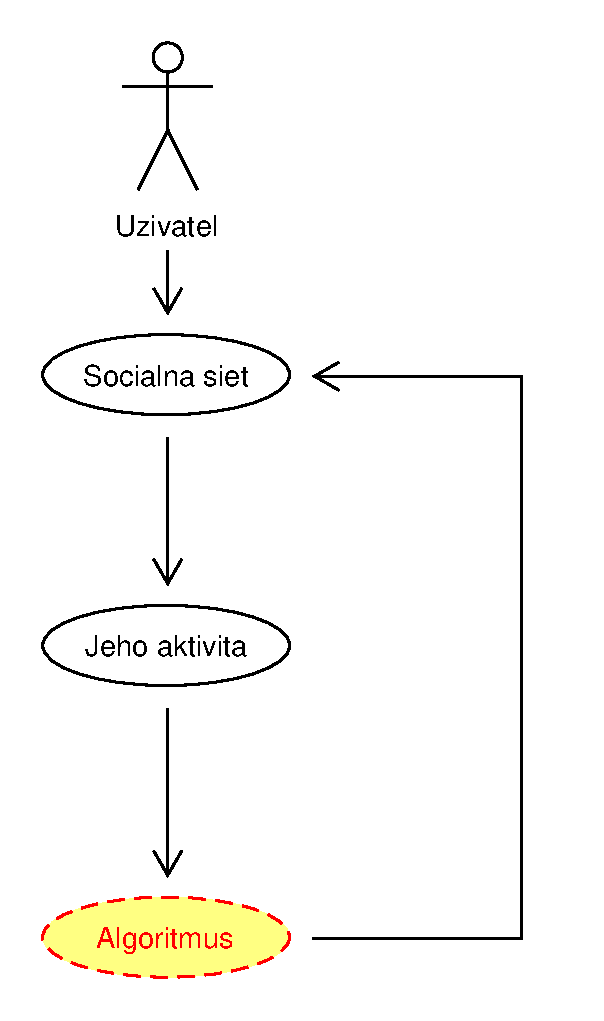
\includegraphics[width=\linewidth]{diagram2.pdf}
        \caption{Obrázok 1}
        \label{fig:obrazok1}
    \end{subfigure}
    \hfill
    \begin{subfigure}{0.45\textwidth}
        \centering
        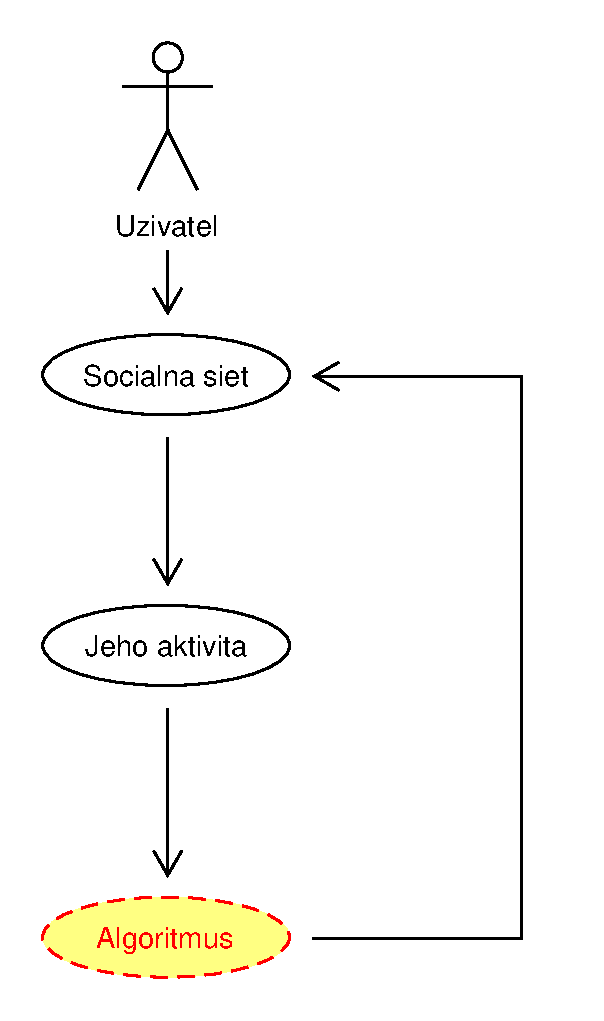
\includegraphics[width=\linewidth]{diagram2.pdf}
        \caption{Obrázok 2}
        \label{fig:obrazok2}
    \end{subfigure}
    \caption{Dva obrázky vedľa seba}
    \label{fig:obrazky-vedla-seba}
\end{figure}

\begin{multicols}{2}

\begin{figure}[H]
      \centering
      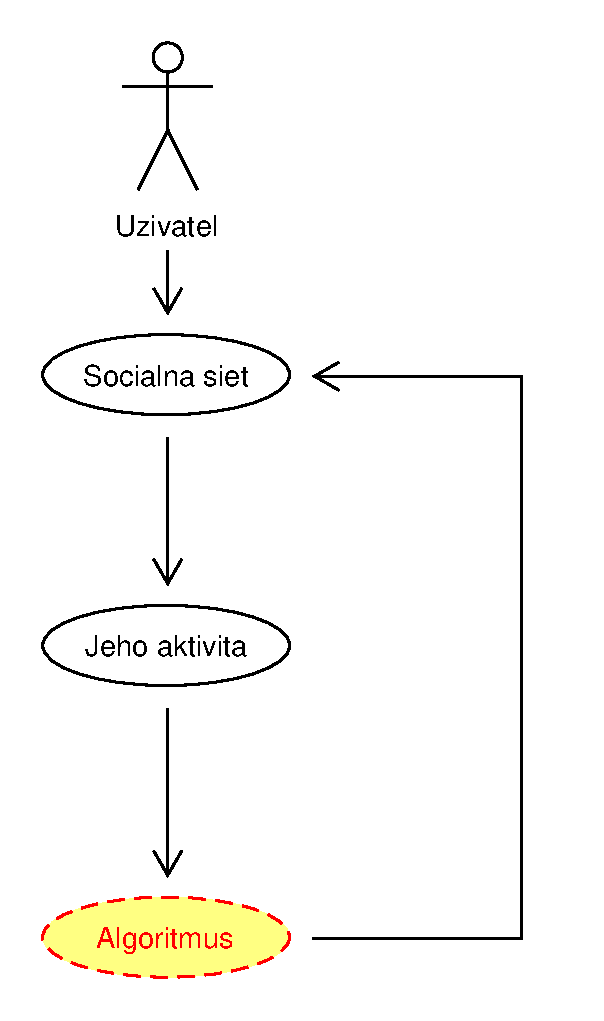
\includegraphics[width= 2\linewidth]{diagram2.pdf}
      \caption{Obrázok na celú šírku}
      \label{fig:obrazok1}
\end{figure}

\end{multicols}

\section{Iná časť} \label{ina}


Môže sa zdať, že problém vlastne nejestvuje\cite{Coplien:MPD}, ale bolo dokázané, že to tak nie je~\cite{Czarnecki:Staged, Czarnecki:Progress}. Napriek tomu, aj dnes na webe narazíme na všelijaké pochybné názory\cite{PLP-Framework}. Dôležité veci možno \emph{zdôrazniť kurzívou}.






%\acknowledgement{Ak niekomu chcete poďakovať\ldots}


% týmto sa generuje zoznam literatúry z obsahu súboru literatura.bib podľa toho, na čo sa v článku odkazujete
\bibliography{literatura}
\bibliographystyle{plain} % prípadne alpha, abbrv alebo hociktorý iný
\end{document}
